%!TEX root = main.tex
\chapter{Background}

This chapter gives a background on the TaleBlazer project, including its separate components and how they work together as a whole. The history of TaleBlazer and past location-based projects are also detailed. Finally, the chapter expands on the need for TaleBlazer Analytics.

\section{TaleBlazer}

TaleBlazer is an augmented reality location-based game platform developed at the MIT Scheller Teacher Education Program (STEP). TaleBlazer is a platform in the true sense in that it is composed of multiple technologies which all come together to produce the TaleBlazer experience. At its core, TaleBlazer lets users create their own games that take place in the real world, using a web-based game editor. Users can then choose to publish their games to the world at large. Using the Android or iOS TaleBlazer mobile application, players play TaleBlazer games by downloading the game and physically walking around in the real-world location that the game takes place in. Players interact with with virtual game agents: user-scripted  entities that are placed by the game designer at specific GPS coordinates.

\subsection{Overview of a TaleBlazer Game}

A typical TaleBlazer game consists of the following parts: 
	\begin{itemize}
		\item regions, which are the real-world locations where the game takes place
		\item roles, which encompass different sets of behaviors for the player(s) in the game
		\item scenarios, which encompass different versions of a game
		\item agents, which are in-game virtual entities that player(s) interact with
		\item traits, variables that belong to different in-game entities or the world
		\item scriptblocks, sets of programming instructions that define the behaviors for game entities
	\end{itemize}

\subsubsection{Regions}

Regions are real-world locations where TaleBlazer games take place. Using the game editor, game designers define their game regions by selecting an area of a Google map. Regions define the area where in-game virtual entities, called agents, can be placed. Games can have one or more regions, each with their own name. The game designer also has the option of moving the player or agents from one region to another during the course of game using TaleBalzer's programming language. In order to play a TaleBlazer game, a player goes to the real-world location with their mobile device and moves around the region to activate or ``bump'' into the agents placed at nearby locations. 

\subsubsection{Roles}

Roles allow game designers to define different characters or types of interactions for different sets of players. This allows designers to create role-playing game experiences. A game can have one or more roles. If a single role is defined, then all players experience the same game. Multiple roles let the game designer define different sets of behaviors for different roles. Each role has a name and an optional description, which players see when choosing between roles at the start of a TaleBlazer game. For example, a game might have players choose between the roles of ``Secret Agent'' and ``Police Officer''.

\subsubsection{Scenarios}

Scenarios allow game designers to create different versions of the same game that players can choose between. For example, scenarios could be difficulty options, such as ``Easy'', ``Medium'', and ``Hard''. Games can have one or more scenarios, each with their own name. If a game has multiple scenarios, then the player is asked to choose between them at the start of a game. The game designer can tailor the behaviors of his game according to the choice of scenario. 

\subsubsection{Agents}

Agents are the in-game virtual entities with which players interact during the course of a TaleBlazer game. Agents have a name, description, set of behaviors, and an optional real-world location. Agents could be anything from items like a treasure chest to a non-player character (NPC) that gives a player quests. Users have multiple methods by which they can interact with agents. Agents placed within a region have corresponding GPS coordinates. Players interact with the agent by arriving at the GPS coordinates of an agent. Some games allow the user to tap on an agent's icon on the map of the game to interact with the agent, referred to as ``tap-to-visit''. Although there are many different ways that a player could come to interact with an agent, an agent interaction in general is referred to as an agent bump.

\subsubsection{Traits}

Traits are variables that can be attached to agents, roles, or the game world in general. Traits have names and values and can be modified during the course of a game based on the behaviors defined by the game designer. Game designers can create their own custom traits, each with a user-defined value. Traits can be used to represent game mechanics, such as a score.

\subsubsection{ScriptBlocks}

ScriptBlocks is a block-based programming language that allows game designers to define the behaviors for their game. ScriptBlocks is block-based because all programming instructions come in the form of blocks that you connect together using a visual game editor (see Figure \ref{fig:game_editor}). For example, conditional behaviors can be defined using a conditional IF-ELSE block, which has sockets that allow you to insert other blocks to define the conditional statement to evaluate. Game designers can write game behaviors by creating agent or role-specific scripts, or by writing scripts applicable to the entire game world. 

TaleBlazer contains a comprehensive set of programming blocks, encompassing a variety of purposes from logical and mathematical functions to TaleBlazer-specific commands. For example, a user can easily check the state of a game agent or move an agent or player from one location to another.

\medskip
\begin{figure}[hbt]
	\center{
			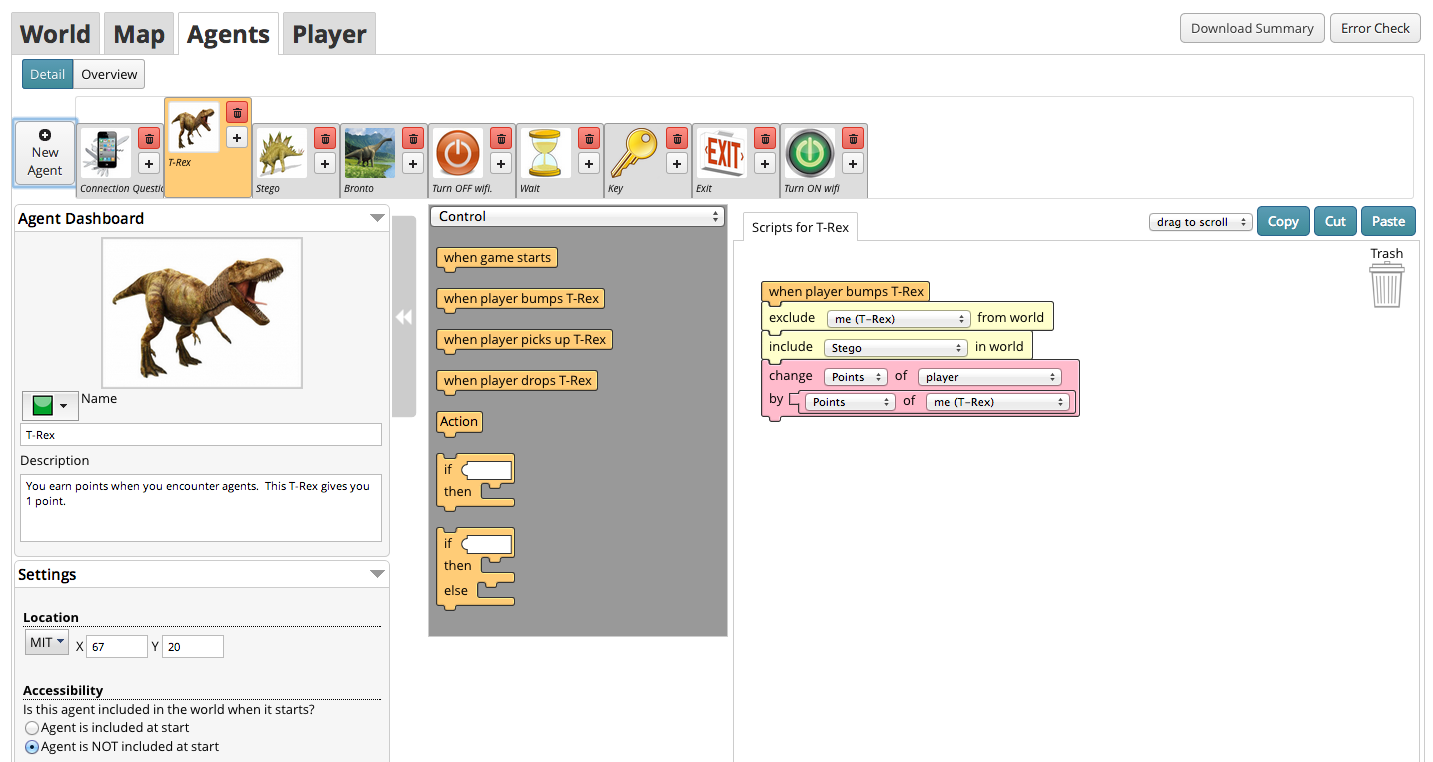
\includegraphics[width=\textwidth]
				{figures/game_editor.png}
			}
	\caption[TaleBlazer Game Editor]{\label{fig:game_editor} The TaleBlazer Game Editor web application}
\end{figure}
\pagebreak

\subsection{TaleBlazer Technology}

The TaleBlazer platform is comprised of four main parts:
	\begin{itemize}
 		\item the game editor, which lets users create their own games
 		\item the mobile application, on which TaleBlazer games are played
 		\item the repository server, which stores and serves games
 		\item and the multiplayer server, which enables multiplayer TaleBlazer games
 	\end{itemize}

\subsubsection{Game Editor}
The game editor is an online web application which lets users create their own TaleBlazer games through the use of ScriptBlocks. Using the editor, users add and configure their game regions, create agents, roles and scenarios, and program the game by composing scripts. Users can save their games, which are then stored on TaleBlazer Server. The game editor also provides options for modifying the game interface that players see when playing a game on their mobile device. The game editor is written in JavaScript. 

\subsubsection{TaleBlazer Mobile}

TaleBlazer Mobile is an Android and iOS mobile application that lets users play TaleBlazer games. The app lets users download TaleBlazer games onto their device and play them, utilizing the location-aware functionalities of the device. TaleBlazer Mobile interprets the blocks in each game file and executes them during the course of the game.

The TaleBlazer Mobile game interface consists primarily of a map of the current game region and icons indicating the position of the player and active game agents (see Figure \ref{fig:app_ui}). Tabs along the top of the screen provide different gameplay functionalities. For example, a game can include the Inventory tab, which tracks currently held items, or the Log tab, which contains a log of all the actions a player has taken during the course of a game.

TaleBlazer Mobile is written using Appcelerator Titanium, an SDK that lets developer write native Android and iOS applications using JavaScript. 

\medskip
\begin{figure}[htb]
	\center{
			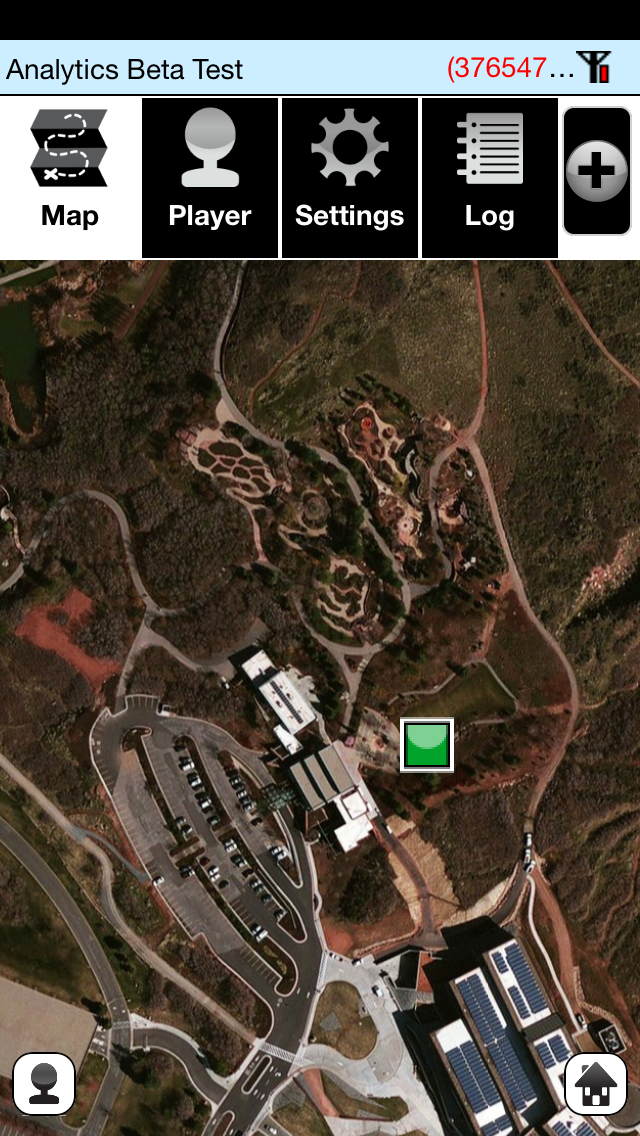
\includegraphics[scale=0.3]
				{figures/app_ui.png}
			}
	\caption[TaleBlazer Mobile Map UI]{\label{fig:app_ui} The TaleBlazer Mobile Main Map Interface}
\end{figure}

\subsubsection{TaleBlazer Server}

TaleBlazer Server is the main repository server which handles user accounts, hosts the game editor, and stores and serves TaleBlazer games and game-related files (e.g. images, video). TaleBlazer Server is written in PHP using the CakePHP framework and backed by a MySQL database. 

\subsubsection{TaleBlazer Multiplayer}

TaleBlazer Multiplayer is a separate server which provides multiplayer functionality for TaleBlazer games. It implements a separate protocol which synchronizes the state of the world between all devices playing a multiplayer game. The server is written in Node.js, using JavaScript.

\subsection{Past Projects}

TaleBlazer is the most recent iteration and study into AR games performed at the STEP lab. Past projects, such as MITAR and StarLogo TNG, provided a basis on which TaleBlazer was built, namely the emphasis on augmented reality and the use of a block-based scripting language.

\subsubsection{MITAR}

MITAR (MIT Augmented Reality) was the immediate ancestor of TaleBlazer. Similar to TaleBlazer, MITAR sought to let users play location-based augmented reality games on earlier mobile platforms, such as Windows Mobile. MITAR also focused on the educational impact of augmented reality games on users. One game, called ``Environmental Detectives'', put users into the roles of investigators searching for the source of a toxic spill, taking measurements in order to determine the environmental impact. \cite{site:ed}

\subsubsection{StarLogo TNG}

StarLogo TNG (The Next Generation) was a project in programmable simulation modeling which allowed users to explore the workings of complex decentralized systems, such as ant colonies and traffic jams. \cite{site:starlogo} Similar to TaleBlazer, users could program the simulation using a block-based scripting language. 

\section{Why Build TaleBlazer Analytics?}

The educational focus of the TaleBlazer project requires that the impact of TaleBlazer games on learning be measured. Game designers and educational researchers are supremely interested in seeing exactly how players play their games in order to draw conclusions as to their games' success and impact.

The rationale behind building TaleBlazer Analytics is two-fold. First, the public release of TaleBlazer requires an automated way of gathering quantitative data about all gameplay sessions. Previously, the only way to gather data was by observing players as they played. Second, existing analytics solutions fail to provide analytics relevant to TaleBlazer with a desirable level of privacy. To this end, it was necessary to build TaleBlazer Analytics to meet our requirements.

\subsection{Purpose of Data Collection}

The overall purpose of collecting TaleBlazer gameplay metrics is to provide interested parties with information to make informed decisions regarding the effectiveness of their game, across different aspects. Specifically, these parties are interested in quantitative metrics, such as the number of players that completed a game and the choices that were made during a gameplay session. 

This type of data could be used to identify buggy game scripts or points of player confusion. It could also be used to determine the appeal of specific narrative elements. For example, a game designer would be able to determine if changing the name of a role from ``Police Officer'' to ``Officer Awesome'' made the role more appealing.

There are four main parties that are interested in this type of data: 
	\begin{itemize}
		\item Game designers
		\item Educational researchers
		\item TaleBlazer developers
		\item Institutions
	\end{itemize}

\subsubsection{Game designers}
Game designers are primarily interested in seeing how players progress through the game and the choices they make along the way. Using this information, a game designer can quickly identify problematic spots. For example, players may stop playing after a particular point in the game because the instructions to proceed aren't clear or there is a bug in the game scripts. As a result, the game designer can improve the game to make it a better experience for the players.

\subsubsection{Educational researchers}

Educational researchers are interested in seeing how a game's content affects a player in the short or long-term. The choices that a player makes during a session can inform the researcher as to the level of a player's knowledge or how the content affected the player's understanding of the topic at hand. The gameplay metrics can be paired with external data, such as post-gameplay questionnaires or interviews. For example, a researcher studying a game about the environment might look at if a player encountered an EPA agent in-game or how fast they completed the game to see if a player missed crucial information or may not have been paying attention. Games can also include in-game research questions, asking players' about their motivation for future activities and their interest in certain educational topics.

\subsubsection{TaleBlazer developers}

TaleBlazer developers are interested in the technical aspects of games in order to inform future technical decisions and feature roadmaps. For example, the kinds of devices being used and the version of their operating systems (OS) are supremely useful in determining possible technical issues related to specific devices and the adoption rate of new OS versions. This information can then be applied to guide the TaleBlazer development process and provide concrete data with which to prioritize tasks. 

\subsubsection{Institutions}

Analytics data may also be used for purposes outside of games. TaleBlazer is currently in use at several institutions across the country, such as botanical gardens, zoos, and historical sites. In these cases, quantitative metadata concerning when and how long games are played can prove especially useful in determining the effectiveness and impact of TaleBlazer games on visitors. Additionally, it can also help provide information about the impact of exhibits and areas of an institution. 

Institutions may be particularly interested in raw numbers, such as how many visitors played a particular game and the game's popularity over time. This can help institutions determine how funding gets spent to improve exhibits and areas. Furthermore, it can also help them identify ways to reach particular hard-to-reach audiences, such as ``tweens''.

\subsection{Motivations}
The user-generated nature of TaleBlazer games results in games that span a huge range of possibilities. As a result, TaleBlazer requires an analytics solution that is both \textit{comprehensive} and \textit{useful}: comprehensive in order to accommodate the range of possibilities of TaleBlazer games, and useful in order to provide meaningful and relevant analytics. In particular, an automated and non-interfering data collection system was necessary in order to collect comprehensive data; a custom analytics system was necessary in order to provide statistics custom and specific to TaleBlazer games.

\subsubsection{Automated Non-Interfering Data Collection}

With the public release of TaleBlazer, it was necessary to automate the collection of data from all gameplay sessions. Previously, all TaleBlazer games were played in a moderated setting, in which adult facilitators would guide gameplay, troubleshoot, and see how the game was being played in real-time. This approach is infeasible when groups are unmoderated or large. As a result, it was necessary to develop an automated system for collecting gameplay data for all sessions.

The previous method for collecting gameplay data involved observing players as they played. Although this approach yielded (and continues to yield) important data regarding players' dialogues and moods, it had two downsides. First, it resulted in an incomplete picture of an entire group's gameplay sessions as the number of players that could be observed was limited to the number of facilitators present. Second, it interfered with gameplay. Players tended to act completely differently when being observed than when left to their own devices, resulting in skewed data. As such, an automated system was nececessary in order to gather quantitative data about all gameplay sessions without interrupting players and to complement existing manual observation methods.

\subsubsection{Relevant Analytics and Privacy}

Existing analytics services were investigated to see if they fit the needs of the TaleBlazer project. These services focus on providing a general data collection solution for its users. Solutions provided by Flurry and Mixpanel, for example, focus on an event-based method of analytics, which tracks unique events across every use of the app. However, these services cannot generate data analytics that are useful and specific to TaleBlazer because they focus on collecting data rather than providing application-specific data analysis. As a result, it was necessary to develop an analytics system built with TaleBlazer in mind. Specifically, this means that features such as data collection, categorization, and statistics calculation can be customized to fit the use cases of TaleBlazer Analytics users. 

A separate concern arose when dealing with the nature of the TaleBlazer analytics data and the question of privacy. Privacy is supremely important to the TaleBlazer project, as games are often played by minors and students. As a result, it is a requirement that any collected data be completely anonymized and only used for educational and research purposes. Existing solutions, such as Flurry, do not guarantee the absolute privacy of the data provided to them and in fact may share that data with third parties. \cite{site:flurry} As such, it was necessary to build TaleBlazer Analytics to ensure that data was anonymized and used only for the purposes of the TaleBlazer project. 





















